\documentclass[]{article}
\usepackage{graphicx} % for pdf, bitmapped graphics files
\begin{document}



\title{Modification of Guidance Law}
\author{Vladimir N. Dobrokhodov}
\date{03/20/2013}
\maketitle

The objective of this new modification is to ``eliminate'' the coordinated turn assumption that is currently used to transform the commanded body rates of the kinematic path following algorithm into the bank angle command used at the input of the autopilot. Overall goal is to improve the path following performance without over constraining the flight.

For the sake of simplicity the proposed approach assumes the following structure of an idealized lateral channel, see Figure~\ref{fig:LatAP}. Here we recognize two major contributors to the commanded roll angle. 
 
\begin{figure}[thpb]
      \centering
      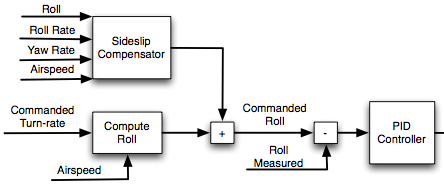
\includegraphics[width=95mm]{APLateral.png}
      \caption{Simplified diagram of lateral channel}
      \label{fig:LatAP}
   \end{figure}
The first one is based on the coordinated turn assumption and uses well-known kinematic expression connecting the turn rate $\dot{\psi}_{cmd}$ with the roll angle $\phi_{crd}$. 

\begin{equation}
\label{eq:coordturn}
	\phi_{crd}=arctan( \frac { \dot{\psi}_{cmd} \cdot V_a} {g})	
\end{equation}
The second component is the compensation necessary to account for the non-zero pitching motion of airplane if the turn is not coordinated. Thus, if the lateral maneuver is not coordinated then there should be some difference in the commanded turn rate that is cased by the nonzero pitch rate $q$ and the pitch angle $\theta$. To calculate the resulting turn rate with the roll angle calculated from eq.\ref{eq:coordturn} we use third Euler attitude kinematic equation

\begin{equation}
\label{eq:psidot}
	\dot{\psi}=\frac {q \cdot sin(\phi_{crd})+ r \cdot cos(\phi_{crd})} {cos(\theta)}	
\end{equation}

Let the error between the turn rates corresponding to the nominal coordinated turn $\dot{\psi}_{cmd}$ and free turning flight with commanded $\phi_{crd}$ be defined as:

\begin{equation}
\label{eq:psierr}
	\dot{\psi}_{err}=\frac { g \cdot tan(\phi_{crd})} {V_a} - \frac {q \cdot sin(\phi_{crd})+ r \cdot cos(\phi_{crd})} {cos(\theta)}	
\end{equation}
This error is the difference that needs to be eliminated when computing the desired bank angle command; as before we utilized the assumption of small angle of attack and side-slip. We propose two approaches to this task. 

Approach 1. Calculate the error $\dot{\psi}_{err}$ as in eq.\ref{eq:psierr} and reuse the coordinated turn relation eq.\ref{eq:coordturn} to calculate the compensating value of additional roll angle.

Approach 2. If the goal is to eliminate the $\dot{\psi}_{err}$ error then resolve the eq.\ref{eq:psidot} with respect the desired roll angle $\phi=\phi_d$ and the actual pitching motion and commanded $\dot{\psi}_{cmd}$.

\end{document}